\documentclass[aspectratio=169,11pt]{beamer}

% ================================================================
% "TABIIY TILNI QAYTA ISHLASH" KURSI
% MA'RUZA 5 --- Ehtimollik modellari: N-grammalar va so'z turkumlarini teglash
%              (d05_til_modellari.tex)
% Arxetiplar: [A][B][C][D][E] + 4 tsikl [F][G][H][I][J][K][L] +
%             [M][N][O][P][Q][R] + ilova [S]
% Rendered slayd soni: ~45 (2-haftaning birinchi ma'ruzasi; L1-L4 chuqurligi)
% Qulflangan [I4]: Viterbi delta(VB, t=2) = 0.3402, ketma-ketlik [NN, VB]
%   --- P5 (Day 6) birinchi assert manbayi (course_map hand_example).
% ================================================================

% ================================================================
% RANGLAR  (asl fayldan o'zgarishsiz)
% ================================================================
\definecolor{cnublue}{rgb}{0.07,0.14,0.62}
\definecolor{cnubluelight}{rgb}{0.18,0.30,0.72}
\definecolor{cnubluebg}{rgb}{0.90,0.92,0.97}
\definecolor{deepblue}{rgb}{0.07,0.14,0.62}
\definecolor{deepred}{rgb}{0.60,0.00,0.00}
\definecolor{deepgreen}{rgb}{0.00,0.45,0.00}
\definecolor{halfgray}{gray}{0.55}

% ================================================================
% BEAMER MAVZU --- Boadilla + maxsus footer  (asl fayldan o'zgarishsiz)
% ================================================================
\usetheme{Boadilla}

\setbeamercolor{structure}{fg=cnublue}
\setbeamercolor{frametitle}{bg=cnublue,fg=white}
\setbeamercolor{title}{bg=cnublue,fg=white}
\setbeamercolor{block title}{bg=cnublue,fg=white}
\setbeamercolor{block body}{bg=cnubluebg,fg=black}
\setbeamercolor{alerted text}{fg=deepred}
\setbeamercolor{author in head/foot}{bg=cnubluelight,fg=white}
\setbeamercolor{section in head/foot}{bg=cnublue,fg=white}
\setbeamercolor{page number in head/foot}{bg=cnubluelight,fg=white}

\setbeamertemplate{mini frame}{}
\setbeamertemplate{mini frame in current section}{}
\setbeamertemplate{mini frame in current subsection}{}
\setbeamertemplate{headline}{}
\setbeamertemplate{navigation symbols}{}

\setbeamertemplate{footline}{%
  \leavevmode%
  \hbox{%
    \begin{beamercolorbox}[wd=0.17\paperwidth,ht=2.5ex,dp=1.25ex,leftskip=0.5em]{author in head/foot}%
      \usebeamerfont{author in head/foot}\scriptsize\insertshortauthor%
    \end{beamercolorbox}%
    \begin{beamercolorbox}[wd=0.69\paperwidth,ht=2.5ex,dp=1.25ex,center]{section in head/foot}%
      \usebeamerfont{section in head/foot}%
      \scriptsize\insertsectionnavigationhorizontal{0.69\paperwidth}{}{}%
    \end{beamercolorbox}%
    \begin{beamercolorbox}[wd=0.14\paperwidth,ht=2.5ex,dp=1.25ex,rightskip=0.5em]{page number in head/foot}%
      \hfill\scriptsize\color{white}%
      \insertframenumber{}/\inserttotalframenumber%
    \end{beamercolorbox}%
  }%
  \vskip0pt%
}

% ================================================================
% PAKETLAR  (asl fayldan o'zgarishsiz)
% ================================================================
\usepackage[utf8]{inputenc}
\usepackage[T1]{fontenc}
\usepackage{lmodern}
\usepackage{amsmath,amssymb}
\usepackage{booktabs}
\usepackage{xcolor}
\usepackage{listings}
\lstset{
    language=Python,
    basicstyle=\ttfamily\scriptsize,
    keywordstyle=\bfseries\color{deepblue},
    emphstyle=\ttfamily\color{deepred},
    stringstyle=\color{deepgreen},
    commentstyle=\itshape\color{halfgray},
    numbers=left,
    numberstyle=\scriptsize\color{halfgray},
    rulesepcolor=\color{cnublue!30},
    frame=shadowbox,
    breaklines=true,
    showstringspaces=false,
    tabsize=2
}
\usepackage{tcolorbox}
\tcbuselibrary{skins}
\tcbset{
  defbox/.style={colback=cnubluebg,colframe=cnublue,
                 fonttitle=\small\bfseries\color{white},
                 attach boxed title to top left={yshift=-2mm,xshift=4mm},
                 boxed title style={colback=cnublue,colframe=cnublue}},
  warnbox/.style={colback=orange!8,colframe=orange!70!black,
                  fonttitle=\small\bfseries},
  okbox/.style={colback=green!7,colframe=green!55!black,
                fonttitle=\small\bfseries}
}
\usepackage{tikz}
\usetikzlibrary{arrows.meta,positioning}

% ================================================================
% QO'SHIMCHALAR  (asl fayldan o'zgarishsiz)
% ================================================================
\AtBeginSection[]{%
  \begin{frame}{Prezentatsiya rejasi}
    \tableofcontents[currentsection]
  \end{frame}}

\newcommand{\bunda}[1]{{\small\textbf{bunda:}\; #1}}
\newcommand{\bajarildi}{{\color{deepgreen}\large$\checkmark$}\;}

% ================================================================
% METAMA'LUMOT
% ================================================================
\title[N-gram va teglash]{Ehtimollik modellari: N-grammalar va so'z turkumlari}
\subtitle{Tabiiy tilni qayta ishlash --- 5-ma'ruza}
\author[A.A.\,Abdulali]{A.A.\,Abdulali}
\date{22-iyun 2026}
\institute{11:00--12:20 \quad$\cdot$\quad mavzu \textnumero{}5}

% ================================================================
\begin{document}
% ================================================================

% ----------------------------------------------------------------
% [A] TITUL
% ----------------------------------------------------------------
\maketitle

% ================================================================
\section[Kirish]{Kirish: matnni ehtimollik bilan modellaymiz}
% ================================================================

% ----------------------------------------------------------------
% [B] TAKRORLASH: L4 va bugungi P4
% ----------------------------------------------------------------
\begin{frame}{Takrorlash: o'tgan darsdan ikki savol}
  \begin{columns}[T]
    \begin{column}{0.49\textwidth}
      \begin{tcolorbox}[warnbox,title=1-savol]
        \small
        L4 noisy channel da $\hat{w}=\arg\max P(x{\mid}w)\,P(w)$ edi.
        Bu yerdagi $P(w)$ --- ``til modeli'' --- bir so'z ehtimoli nechanchi
        tartibli N-gram?
      \end{tcolorbox}
    \end{column}
    \begin{column}{0.49\textwidth}
      \begin{tcolorbox}[warnbox,title=2-savol]
        \small
        P4 da \texttt{edit\_distance} dinamik dasturlash (DP) bilan
        hisoblandi. Bugungi Viterbi ham DP --- sizningcha nega ikkalasi DP?
      \end{tcolorbox}
    \end{column}
  \end{columns}
  \pause
  \vspace{4pt}
  \begin{columns}[T]
    \begin{column}{0.49\textwidth}
      \begin{tcolorbox}[okbox,title=1-javob]
        \small
        \textbf{Unigram} (1-gram) --- so'z chastotasi. Bugun uni
        bigram/trigramga kengaytiramiz: kontekstni hisobga olamiz.
      \end{tcolorbox}
    \end{column}
    \begin{column}{0.49\textwidth}
      \begin{tcolorbox}[okbox,title=2-javob]
        \small
        Ikkalasi ham masalani \textbf{kichik qism-masalalar}ga bo'lib,
        ularning optimal yechimidan butunni quradi --- DP mohiyati.
      \end{tcolorbox}
    \end{column}
  \end{columns}
\end{frame}

% ----------------------------------------------------------------
% [C] MAQSADLAR
% ----------------------------------------------------------------
\begin{frame}{Siz bugungi dars oxirida quyidagilarni bajara olasiz:}
  \begin{enumerate}\setlength\itemsep{6pt}
    \item \textbf{Keltirib chiqara olasiz:} bigram ehtimolini sanash asosida
          (MLE) --- zanjir qoidasi va Markov taxminidan.
    \item \textbf{Hisoblay olasiz:} add-1 (Laplace) smoothing va perplexity ni
          kichik korpusda qo'lda.
    \item \textbf{Qo'llay olasiz:} Markov zanjiri bilan teg ketma-ketligi
          ehtimolini.
    \item \textbf{Keltirib chiqara olasiz:} Viterbi DP bilan eng ehtimoliy teg
          ketma-ketligini ($\delta(\text{VB},t{=}2)=0.3402$).
  \end{enumerate}
  \vspace{4pt}
  \begin{tcolorbox}[defbox,title=Oldindan talab]
    \footnotesize
    L2 dan: ehtimollik, $\arg\max$, log. L4 dan: dinamik dasturlash, til modeli
    $P(w)$. Matematikadan: ko'paytma, maksimum.
  \end{tcolorbox}
\end{frame}

% ----------------------------------------------------------------
% [D] REJA
% ----------------------------------------------------------------
\begin{frame}{Bugungi dars rejasi:}
  \begin{center}
  \small
  \begin{tabular}{c p{5.2cm} c p{3.0cm}}
    \toprule
    \textbf{Tsikl}& \textbf{Mavzu} & \textbf{Vaqt} & \textbf{Hosil bo'luvchi natija}\\
    \midrule
    1 & N-gram til modeli (uni/bi/trigram) & 18 daq & $P(\text{kitob}{\mid}\text{men})=2/3$ \\
    2 & Perplexity va smoothing & 18 daq & Add-1, perplexity \\
    3 & So'z turkumlari (POS) + Markov & 14 daq & $P(\text{NN},\text{VB})=0.42$ \\
    4 & Yashirin Markov + Viterbi & 20 daq & $\delta(\text{VB},t{=}2)=0.3402$ \\
    \midrule
      & Xulosa va 5-amaliyotga ko'rsatmalar & 10 daq & Ertaga nima qurishingiz \\
    \bottomrule
  \end{tabular}
  \end{center}
  \vspace{4pt}
  \begin{tcolorbox}[warnbox,title=Bu dars 2-haftani ochadi]
    \footnotesize\sloppy
    Klassik pipeline (1-hafta) dan ehtimollik modellari (2-hafta) ga o'tamiz.
    Bugungi Viterbi $\delta(\text{VB},t{=}2)=0.3402$ ertangi P5 da \texttt{assert} bo'ladi.
  \end{tcolorbox}
\end{frame}

% ----------------------------------------------------------------
% [E] MUAMMO BIRINCHI
% ----------------------------------------------------------------
\begin{frame}{Bugungi dars uchun muammo: ``men \underline{\hspace{0.6cm}}'' dan keyin qaysi so'z keladi?}
  \begin{columns}[T]
    \begin{column}{0.50\textwidth}
      \textbf{Ikki vazifa:}\\[3pt]
      \small
      \begin{tcolorbox}[warnbox,title=1. Avtomatik to'ldirish,top=2pt,bottom=2pt]
        \footnotesize
        Telefon klaviaturasi \texttt{"men"} dan keyin keyingi so'zni taklif
        qiladi. Qaysi so'z eng ehtimoliy?
      \end{tcolorbox}
      \vspace{3pt}
      \begin{tcolorbox}[warnbox,title=2. So'z turkumini aniqlash,top=2pt,bottom=2pt]
        \footnotesize
        \texttt{"yozdi"} --- bu fe'lmi yoki ot? Kontekst hal qiladi.
        Butun gapdagi \textbf{teglar ketma-ketligini} qanday topamiz?
      \end{tcolorbox}
    \end{column}
    \begin{column}{0.46\textwidth}
      \textbf{Bugungi yechimlar:}\\[4pt]
      \small
      \begin{enumerate}\setlength\itemsep{4pt}
        \item \textbf{N-gram til modeli}: oldingi so'z(lar)ga qarab keyingisini
              ehtimollik bilan bashorat qiladi.
        \item \textbf{HMM + Viterbi}: yashirin teglar ketma-ketligining eng
              ehtimoliysini topadi.
      \end{enumerate}
      \vspace{5pt}
      \begin{tcolorbox}[okbox,top=2pt,bottom=2pt]
        \footnotesize
        Ikkalasining yuragida bitta g'oya: \textbf{ehtimollik} va uni
        sanash asosida baholash.
      \end{tcolorbox}
    \end{column}
  \end{columns}
\end{frame}

% ================================================================
\section[N-gram]{N-gram til modellari}
% ================================================================

% ----------------------------------------------------------------
% [F1] INTUITSIYA
% ----------------------------------------------------------------
\begin{frame}{Intuitsiya: keyingi so'zni oldingilariga qarab bashorat qilamiz}
  \begin{columns}[T]
    \begin{column}{0.52\textwidth}
      \small
      \texttt{"men"} $\to$ \texttt{kitob}? \texttt{non}? \texttt{keldim}?\\[4pt]
      Til modeli har bir davom uchun \textbf{ehtimol} beradi va eng yuqorisini
      taklif qiladi.\\[6pt]
      \textbf{Nechta oldingi so'z?}
      \begin{itemize}\setlength\itemsep{1pt}
        \item \textbf{unigram}: kontekstsiz --- $P(w)$
        \item \textbf{bigram}: 1 oldingi --- $P(w_i{\mid}w_{i-1})$
        \item \textbf{trigram}: 2 oldingi --- $P(w_i{\mid}w_{i-2},w_{i-1})$
      \end{itemize}
    \end{column}
    \begin{column}{0.44\textwidth}
      \begin{tcolorbox}[okbox,top=2pt,bottom=2pt]
        \footnotesize
        Ko'proq kontekst $\Rightarrow$ aniqroq bashorat, lekin
        ko'proq ma'lumot kerak (kamdan-kam uchraydigan N-gramlar).
        Bu murosani 2-tsiklda ko'ramiz.
      \end{tcolorbox}
    \end{column}
  \end{columns}
\end{frame}

% ----------------------------------------------------------------
% [G1] RASMIY TA'RIF + BUNDA
% ----------------------------------------------------------------
\begin{frame}{N-gram til modeli: rasmiy ta'rif}
  \begin{tcolorbox}[defbox,title=Ta'rif: bigram ehtimoli (MLE)]
    \vspace{-0.4em}
    $$ P(w_i \mid w_{i-1}) = \frac{\text{count}(w_{i-1}, w_i)}{\text{count}(w_{i-1})} $$
  \end{tcolorbox}
  \vspace{3pt}
  \bunda{$\text{count}(w_{i-1},w_i)$ --- $w_{i-1}$ dan keyin $w_i$ kelgan
  hollar soni; $\text{count}(w_{i-1})$ --- $w_{i-1}$ ning umumiy soni;
  MLE --- maksimal extimollik bahosi (chastotaga asoslangan).}
  \vspace{5pt}
  \textbf{Gap ehtimoli (bigram):}
  $$ P(w_1 \ldots w_n) \approx \prod_{i=1}^{n} P(w_i \mid w_{i-1}) $$
  \footnotesize Trigram: maxrajda 2 so'zli kontekst
  $\text{count}(w_{i-2},w_{i-1})$.
\end{frame}

% ----------------------------------------------------------------
% [H1] KELTIRIB CHIQARISH
% ----------------------------------------------------------------
\begin{frame}{Keltirib chiqarish: zanjir qoidasidan bigramga}
  \textbf{1-qadam.} Zanjir (ehtimollar ko'paytmasi) qoidasi --- aniq:
  $$ P(w_1 \ldots w_n) = \prod_{i=1}^{n} P(w_i \mid w_1 \ldots w_{i-1}) $$
  \pause
  \textbf{2-qadam.} Muammo: $P(w_i \mid w_1\ldots w_{i-1})$ ni sanash mumkin emas
  --- bunday uzun kontekst deyarli takrorlanmaydi (ma'lumot yetmaydi).
  \pause
  \textbf{3-qadam.} \textbf{Markov taxmini}: faqat oxirgi $n{-}1$ so'z muhim:
  $$ P(w_i \mid w_1\ldots w_{i-1}) \approx P(w_i \mid w_{i-1}) \quad(\text{bigram}) $$
  \begin{tcolorbox}[okbox,top=2pt,bottom=2pt]
    \small \textbf{Xulosa:} aniqlikni soddalik va sanaluvchanlikka almashtiramiz.
    Bu --- til modellashtirishning asosiy murosasi.
  \end{tcolorbox}
\end{frame}

% ----------------------------------------------------------------
% [I1] QO'LDA MISOL
% ----------------------------------------------------------------
\begin{frame}{Qo'lda misol: bigram ehtimolini sanaymiz}
  \begin{tcolorbox}[defbox,title=Kichik korpus (3 gap)]
    \small
    $S_1$: \texttt{men kitob o'qidim} \quad
    $S_2$: \texttt{men non yedim} \quad
    $S_3$: \texttt{men kitob oldim}
  \end{tcolorbox}
  \vspace{0.2em}
  \begin{columns}[T]
    \begin{column}{0.52\textwidth}
      \textbf{Sanaymiz:}
      \begin{align*}
        \text{count}(\text{men}) &= 3\\
        \text{count}(\text{men},\text{kitob}) &= 2
      \end{align*}
      $$ P(\text{kitob}\mid\text{men}) = \frac{2}{3} \approx \mathbf{0.667} $$
    \end{column}
    \begin{column}{0.44\textwidth}
      \begin{tcolorbox}[okbox,top=2pt,bottom=2pt]
        \footnotesize
        ``men'' dan keyin \texttt{kitob} (2 marta) \texttt{non} (1 marta) dan
        ko' proq kutiladi $\Rightarrow$ avtomatik to'ldirish \texttt{kitob} ni
        taklif qiladi.
      \end{tcolorbox}
      \vspace{3pt}
      \footnotesize\color{halfgray}
      Bu korpusning lug'at hajmi $|V|=6$
      (men, kitob, o'qidim, non, yedim, oldim).
    \end{column}
  \end{columns}
\end{frame}

% ----------------------------------------------------------------
% [J1] SIZNING VAZIFANGIZ
% ----------------------------------------------------------------
\begin{frame}{Sizning vazifangiz: yana bir bigram}
  \begin{tcolorbox}[warnbox,title=Savol --- 90 soniya]
    \small
    Xuddi shu korpus ($S_1,S_2,S_3$) uchun:\\[4pt]
    \textbf{\large $P(\text{non}\mid\text{men}) = ?$}
  \end{tcolorbox}
  \pause
  \begin{tcolorbox}[okbox,title=Javob]
    \small
    $\text{count}(\text{men},\text{non}) = 1$, \quad $\text{count}(\text{men}) = 3$\\[3pt]
    $P(\text{non}\mid\text{men}) = \dfrac{1}{3} \approx \mathbf{0.333}$\\[3pt]
    \footnotesize Tekshiruv: $P(\text{kitob}{\mid}\text{men}) + P(\text{non}{\mid}\text{men})
    = 2/3 + 1/3 = 1$ --- ``men'' dan keyin faqat shu ikki so'z kelgan.
  \end{tcolorbox}
\end{frame}

% ----------------------------------------------------------------
% [K1] KOD <-> FORMULA  [fragile]
% ----------------------------------------------------------------
\begin{frame}[fragile]{Kod $\leftrightarrow$ formula: bigram modeli}
  \begin{columns}[T]
    \begin{column}{0.56\textwidth}
\begin{lstlisting}
from collections import Counter

corpus = [["men", "kitob", "o'qidim"],
          ["men", "non", "yedim"],
          ["men", "kitob", "oldim"]]

uni = Counter(w for s in corpus for w in s)
bi = Counter((s[i], s[i+1])
             for s in corpus
             for i in range(len(s) - 1))

def p_bigram(prev, w):
    return bi[(prev, w)] / uni[prev]

print(p_bigram("men", "kitob"))   # 0.667
\end{lstlisting}
    \end{column}
    \begin{column}{0.40\textwidth}
      \textbf{Kod $\to$ formula:}\\[3pt]
      \footnotesize
      \begin{tabular}{p{2.0cm}p{2.0cm}}
        \toprule
        Kod & Formula \\
        \midrule
        \texttt{bi[(prev,w)]} & $\text{count}(w_{i-1},w_i)$ \\
        \texttt{uni[prev]} & $\text{count}(w_{i-1})$ \\
        \texttt{bi/uni} & $P(w_i{\mid}w_{i-1})$ \\
        \bottomrule
      \end{tabular}
      \vspace{4pt}
      \begin{tcolorbox}[okbox,top=2pt,bottom=2pt]
        \footnotesize
        Ertangi P5 da \texttt{m05 Autocomplete} aynan shu sanashga tayanadi.
      \end{tcolorbox}
    \end{column}
  \end{columns}
\end{frame}

% ----------------------------------------------------------------
% [L1] TUZOG'
% ----------------------------------------------------------------
\begin{frame}{N-gram tuzog'i: ko'rilmagan birikma butun gapni nolga aylantiradi}
  \begin{columns}[T]
    \begin{column}{0.52\textwidth}
      \begin{tcolorbox}[warnbox,title=Nol muammosi (zero problem)]
        \small
        Test gapi: \texttt{"men non o'qidim"}.\\[3pt]
        $(\text{non},\text{o'qidim})$ korpusda \textbf{hech uchramagan}
        $\Rightarrow P=0$.\\[3pt]
        Bigram ko'paytmada bitta $0$ $\Rightarrow$ \textbf{butun gap} ehtimoli
        $= 0$.
      \end{tcolorbox}
    \end{column}
    \begin{column}{0.44\textwidth}
      \footnotesize
      Bu jiddiy: model ko'rmagan har qanday yangi birikmani ``imkonsiz'' deb
      hisoblaydi --- til esa cheksiz ijodiy.\\[4pt]
      \textbf{Yechim:} \textit{smoothing} --- ko'rilmagan birikmaga ham kichik
      ehtimol beramiz (2-tsikl).
    \end{column}
  \end{columns}
\end{frame}

% ================================================================
\section[Perplexity]{Perplexity va smoothing}
% ================================================================

% ----------------------------------------------------------------
% [F2] INTUITSIYA
% ----------------------------------------------------------------
\begin{frame}{Intuitsiya: model qanchalik ``hayron'' bo'ladi?}
  \begin{columns}[T]
    \begin{column}{0.52\textwidth}
      \small
      \textbf{Perplexity} --- model test matnini ko'rganda qanchalik
      ``hayron'' bo'lishi. Past perplexity $\Rightarrow$ yaxshi model
      (matnni kutgan).\\[6pt]
      Taxminan: model har qadamda \textbf{nechta} teng ehtimolli variant
      orasidan tanlayotgandek. Past son $\Rightarrow$ ishonchli.
    \end{column}
    \begin{column}{0.44\textwidth}
      \begin{tcolorbox}[defbox,title=Smoothing,top=2pt,bottom=2pt]
        \footnotesize
        Ko'rilmagan birikmaga ham \textbf{kichik} ehtimol beramiz ---
        ehtimollik massasining bir qismini ``zaxiraga'' ajratamiz.
        Eng oddiysi: har sanoqqa $+1$ (Laplace).
      \end{tcolorbox}
    \end{column}
  \end{columns}
\end{frame}

% ----------------------------------------------------------------
% [G2] RASMIY TA'RIF + BUNDA
% ----------------------------------------------------------------
\begin{frame}{Perplexity va add-1 (Laplace) smoothing: ta'rif}
  \begin{tcolorbox}[defbox,title=Ta'rif: perplexity]
    \vspace{-0.4em}
    $$ \mathrm{PP}(W) = P(w_1\ldots w_N)^{-\frac{1}{N}}
       = \exp\!\Big(\!-\tfrac{1}{N}\textstyle\sum_{i=1}^{N}\ln P(w_i\mid w_{i-1})\Big) $$
  \end{tcolorbox}
  \vspace{2pt}
  \bunda{$N$ --- test tokenlar soni; past $\mathrm{PP}$ --- yaxshi model;
  bir tekis (uniform) $|V|$ variantli model uchun $\mathrm{PP}=|V|$.}
  \vspace{4pt}
  \begin{tcolorbox}[defbox,title=Ta'rif: add-1 (Laplace) smoothing]
    \vspace{-0.4em}
    $$ P_{+1}(w_i\mid w_{i-1}) = \frac{\text{count}(w_{i-1},w_i) + 1}{\text{count}(w_{i-1}) + |V|} $$
  \end{tcolorbox}
\end{frame}

% ----------------------------------------------------------------
% [H2] KELTIRIB CHIQARISH
% ----------------------------------------------------------------
\begin{frame}{Keltirib chiqarish: nega maxrajga $|V|$ qo'shamiz?}
  \textbf{1-qadam.} Har bigram sanog'iga $+1$ qo'shamiz (ko'rilmaganlar ham
  $0$ emas, $1$ bo'ladi).
  \pause
  \textbf{2-qadam.} Ehtimollar yig'indisi $1$ bo'lishi shart. $w_{i-1}$ dan
  keyin \textbf{har} bir lug'at so'zi ($|V|$ ta) uchun $+1$ qo'shdik:
  $$ \sum_{w}\big(\text{count}(w_{i-1},w)+1\big) = \text{count}(w_{i-1}) + |V| $$
  \pause
  \textbf{3-qadam.} Shuning uchun maxraj $\text{count}(w_{i-1}) + |V|$:
  $$ P_{+1}(w_i\mid w_{i-1}) = \frac{\text{count}(w_{i-1},w_i)+1}{\text{count}(w_{i-1})+|V|} $$
  \begin{tcolorbox}[okbox,top=2pt,bottom=2pt]
    \small \textbf{Xulosa:} massaning bir qismi ko'rilganlardan ko'rilmaganlarga
    ko'chadi --- shuning uchun seen birikma ehtimoli biroz \textbf{pasayadi}.
  \end{tcolorbox}
\end{frame}

% ----------------------------------------------------------------
% [I2] QO'LDA MISOL
% ----------------------------------------------------------------
\begin{frame}{Qo'lda misol: smoothing nol muammosini hal qiladi}
  \begin{tcolorbox}[defbox,title={Test birikmasi: (non, o'qidim) --- korpusda yo'q}]
    \small $|V|=6$, \; $\text{count}(\text{non})=1$, \;
    $\text{count}(\text{non},\text{o'qidim})=0$.
  \end{tcolorbox}
  \vspace{0.2em}
  \begin{columns}[T]
    \begin{column}{0.50\textwidth}
      \textbf{Smoothingsiz:}
      $$ P(\text{o'qidim}\mid\text{non}) = \frac{0}{1} = \mathbf{0} $$
      $\Rightarrow$ gap ehtimoli $0$, \; $\mathrm{PP}=\infty$ \alert{(halokat)}.
    \end{column}
    \begin{column}{0.46\textwidth}
      \textbf{Add-1 bilan:}
      $$ P_{+1}(\text{o'qidim}\mid\text{non}) = \frac{0+1}{1+6} = \frac{1}{7} \approx \mathbf{0.143} $$
      $\Rightarrow$ kichik, ammo \textbf{noldan katta}; $\mathrm{PP}$ chekli.
    \end{column}
  \end{columns}
  \vspace{4pt}
  \begin{tcolorbox}[okbox,top=2pt,bottom=2pt]
    \footnotesize
    Smoothing modelni ``yangilik''ka tayyor qiladi --- ko'rilmagan birikma endi
    butun gapni o'ldirmaydi.
  \end{tcolorbox}
\end{frame}

% ----------------------------------------------------------------
% [J2] SIZNING VAZIFANGIZ
% ----------------------------------------------------------------
\begin{frame}{Sizning vazifangiz: add-1 ehtimolini hisoblang}
  \begin{tcolorbox}[warnbox,title=Savol --- 90 soniya]
    \small
    Xuddi shu korpus ($|V|=6$, $\text{count}(\text{men})=3$,
    $\text{count}(\text{men},\text{kitob})=2$):\\[4pt]
    \textbf{\large $P_{+1}(\text{kitob}\mid\text{men}) = ?$}\\[3pt]
    \footnotesize Smoothingsiz qiymat $2/3$ edi --- add-1 dan keyin qanday o'zgaradi?
  \end{tcolorbox}
  \pause
  \begin{tcolorbox}[okbox,title=Javob]
    \small
    $P_{+1}(\text{kitob}\mid\text{men}) = \dfrac{2+1}{3+6} = \dfrac{3}{9}
       = \dfrac{1}{3} \approx \mathbf{0.333}$\\[3pt]
    \footnotesize Seen birikma ehtimoli $2/3 \to 1/3$ ga \textbf{pasaydi} ---
    massa ko'rilmaganlarga ko'chdi. Bu smoothing narxi.
  \end{tcolorbox}
\end{frame}

% ----------------------------------------------------------------
% [K2] KOD <-> FORMULA  [fragile]
% ----------------------------------------------------------------
\begin{frame}[fragile]{Kod $\leftrightarrow$ formula: add-1 va perplexity}
  \begin{columns}[T]
    \begin{column}{0.56\textwidth}
\begin{lstlisting}
import math

V = len(uni)   # lug'at hajmi = 6

def p_add1(prev, w):
    return (bi[(prev, w)] + 1) / (uni[prev] + V)

def perplexity(pairs):   # pairs: [(prev, w), ...]
    log_sum = sum(math.log(p_add1(a, b))
                  for a, b in pairs)
    return math.exp(-log_sum / len(pairs))

print(p_add1("non", "o'qidim"))   # 1/7 = 0.143
\end{lstlisting}
    \end{column}
    \begin{column}{0.40\textwidth}
      \textbf{Kod $\to$ formula:}\\[3pt]
      \footnotesize
      \begin{tabular}{p{1.9cm}p{2.1cm}}
        \toprule
        Kod & Formula \\
        \midrule
        \texttt{+ 1} & $+1$ (Laplace) \\
        \texttt{+ V} & $+|V|$ \\
        \texttt{-log\_sum/N} & $-\frac1N\sum\ln P$ \\
        \texttt{exp(...)} & $\mathrm{PP}$ \\
        \bottomrule
      \end{tabular}
      \vspace{4pt}
      \begin{tcolorbox}[warnbox,top=2pt,bottom=2pt]
        \footnotesize
        Log fazoda yig'amiz --- ko'paytma underflow ga olib keladi
        (4-tsikl [L]).
      \end{tcolorbox}
    \end{column}
  \end{columns}
\end{frame}

% ----------------------------------------------------------------
% [L2] TUZOG'
% ----------------------------------------------------------------
\begin{frame}{Perplexity tuzog'i: nimani taqqoslayapsiz?}
  \begin{columns}[T]
    \begin{column}{0.50\textwidth}
      \begin{tcolorbox}[warnbox,title=Cheklovlar]
        \small
        \begin{itemize}\setlength\itemsep{2pt}
          \item Perplexity faqat \textbf{bir xil lug'at} va \textbf{bir xil test
                to'plam}da taqqoslanadi.
          \item OOV (lug'atdan tashqari) so'zlar perplexity ni keskin buzadi.
          \item Ortiqcha smoothing taqsimotni tekislaydi --- model
                ``hammasi mumkin'' deydi, foydasi kamayadi.
        \end{itemize}
      \end{tcolorbox}
    \end{column}
    \begin{column}{0.46\textwidth}
      \begin{tcolorbox}[okbox,top=2pt,bottom=2pt]
        \footnotesize
        Past perplexity --- \textbf{vosita}, maqsad emas. Yakuniy vazifadagi
        sifat (masalan to'ldirish to'g'riligi) muhimroq.
      \end{tcolorbox}
      \vspace{3pt}
      \footnotesize\color{halfgray}
      Yaxshiroq usullar: add-$k$, Kneser--Ney, backoff (kurs doirasidan tashqari).
    \end{column}
  \end{columns}
\end{frame}

% ================================================================
\section[POS]{So'z turkumlari va Markov zanjirlari}
% ================================================================

% ----------------------------------------------------------------
% [F3] INTUITSIYA
% ----------------------------------------------------------------
\begin{frame}{Intuitsiya: har so'zga turkum, har turkum oldingisiga bog'liq}
  \begin{columns}[T]
    \begin{column}{0.52\textwidth}
      \small
      \textbf{So'z turkumini aniqlash (POS):} har so'zga teg --- ot (NN),
      fe'l (VB), sifat\ldots\\[4pt]
      \texttt{men}(PR) \; \texttt{kitob}(NN) \; \texttt{o'qidim}(VB)\\[6pt]
      \textbf{Markov g'oyasi:} keyingi teg asosan \textbf{oldingi}
      tegga bog'liq. Otdan keyin ko'pincha fe'l, sifatdan keyin ot\ldots
    \end{column}
    \begin{column}{0.44\textwidth}
      \begin{tcolorbox}[okbox,top=2pt,bottom=2pt]
        \footnotesize
        Bir xil so'z turli teg olishi mumkin: kontekst hal qiladi.
        Markov zanjiri teglar orasidagi \textbf{o'tish}larni modellaydi.
      \end{tcolorbox}
    \end{column}
  \end{columns}
\end{frame}

% ----------------------------------------------------------------
% [G3] RASMIY TA'RIF + BUNDA
% ----------------------------------------------------------------
\begin{frame}{Markov zanjiri: rasmiy ta'rif}
  \begin{tcolorbox}[defbox,title=Ta'rif: 1-tartibli Markov zanjiri]
    \vspace{-0.4em}
    $$ P(s_1 s_2 \ldots s_T) = \pi(s_1)\prod_{t=2}^{T} A(s_t \mid s_{t-1}) $$
  \end{tcolorbox}
  \vspace{3pt}
  \bunda{$s_t$ --- $t$-holat (teg); $\pi(s_1)$ --- boshlang'ich ehtimol;
  $A(s_t\mid s_{t-1})$ --- o'tish (transition) ehtimoli; 1-tartib --- keyingi
  holat faqat \textbf{bitta} oldingisiga bog'liq.}
  \vspace{5pt}
  \textbf{Bizning o'tish matritsasi (NN, VB):}
  \begin{center}\small
  \begin{tabular}{c|cc}
     & $\to$ NN & $\to$ VB \\
    \hline
    NN & 0.4 & 0.6 \\
    VB & 0.3 & 0.7 \\
  \end{tabular}\qquad $\pi(\text{NN})=0.7,\;\pi(\text{VB})=0.3$
  \end{center}
\end{frame}

% ----------------------------------------------------------------
% [H3] KELTIRIB CHIQARISH
% ----------------------------------------------------------------
\begin{frame}{Keltirib chiqarish: to'liq qo'shma ehtimoldan Markovgacha}
  \textbf{1-qadam.} Teglar ketma-ketligining to'liq ehtimoli (zanjir qoidasi):
  $$ P(s_1\ldots s_T) = \pi(s_1)\prod_{t=2}^{T} P(s_t\mid s_1\ldots s_{t-1}) $$
  \pause
  \textbf{2-qadam.} 1-tartibli Markov taxmini --- faqat oldingi holat muhim:
  $$ P(s_t\mid s_1\ldots s_{t-1}) \approx P(s_t\mid s_{t-1}) = A(s_t\mid s_{t-1}) $$
  \pause
  \textbf{3-qadam.} Demak:
  $$ P(s_1\ldots s_T) = \pi(s_1)\prod_{t=2}^{T} A(s_t\mid s_{t-1}) $$
  \begin{tcolorbox}[okbox,top=2pt,bottom=2pt]
    \small Bu --- N-gram bilan \textbf{bir xil g'oya}, faqat so'zlar o'rniga
    teglar ustida.
  \end{tcolorbox}
\end{frame}

% ----------------------------------------------------------------
% [I3] QO'LDA MISOL
% ----------------------------------------------------------------
\begin{frame}{Qo'lda misol: teg ketma-ketligi ehtimoli}
  \begin{tcolorbox}[defbox,title=Ketma-ketlik: NN -> VB]
    \small $\pi(\text{NN})=0.7$, \quad $A(\text{VB}\mid\text{NN})=0.6$.
  \end{tcolorbox}
  \vspace{0.2em}
  \begin{columns}[T]
    \begin{column}{0.50\textwidth}
      \textbf{Hisoblaymiz:}
      \begin{align*}
        P(\text{NN},\text{VB}) &= \pi(\text{NN})\cdot A(\text{VB}\mid\text{NN})\\
          &= 0.7 \times 0.6 = \mathbf{0.42}
      \end{align*}
    \end{column}
    \begin{column}{0.46\textwidth}
      \begin{tcolorbox}[okbox,top=2pt,bottom=2pt]
        \footnotesize
        Bu faqat \textbf{teglar} ehtimoli (so'zlarsiz). Keyingi tsiklda
        so'zlar (kuzatuvlar) qo'shilib, HMM hosil bo'ladi.
      \end{tcolorbox}
    \end{column}
  \end{columns}
\end{frame}

% ----------------------------------------------------------------
% [J3] SIZNING VAZIFANGIZ
% ----------------------------------------------------------------
\begin{frame}{Sizning vazifangiz: teskari ketma-ketlik}
  \begin{tcolorbox}[warnbox,title=Savol --- 60 soniya]
    \small
    $\pi(\text{VB})=0.3$, \quad $A(\text{NN}\mid\text{VB})=0.3$.\\[4pt]
    \textbf{\large $P(\text{VB},\text{NN}) = ?$}
  \end{tcolorbox}
  \pause
  \begin{tcolorbox}[okbox,title=Javob]
    \small
    $P(\text{VB},\text{NN}) = \pi(\text{VB})\cdot A(\text{NN}\mid\text{VB})
       = 0.3 \times 0.3 = \mathbf{0.09}$\\[3pt]
    \footnotesize $0.09 < 0.42$ --- bu korpusda gap \textbf{ot bilan boshlanib
    fe'l bilan davom etishi} ancha ehtimoliyroq (NN$\to$VB).
  \end{tcolorbox}
\end{frame}

% ----------------------------------------------------------------
% [K3] KOD <-> FORMULA  [fragile]
% ----------------------------------------------------------------
\begin{frame}[fragile]{Kod $\leftrightarrow$ formula: Markov ketma-ketligi}
  \begin{columns}[T]
    \begin{column}{0.56\textwidth}
\begin{lstlisting}
pi = {"NN": 0.7, "VB": 0.3}
A = {("NN", "NN"): 0.4, ("NN", "VB"): 0.6,
     ("VB", "NN"): 0.3, ("VB", "VB"): 0.7}

def seq_prob(tags):
    p = pi[tags[0]]
    for i in range(1, len(tags)):
        p *= A[(tags[i-1], tags[i])]
    return p

print(seq_prob(["NN", "VB"]))   # 0.42
print(seq_prob(["VB", "NN"]))   # 0.09
\end{lstlisting}
    \end{column}
    \begin{column}{0.40\textwidth}
      \textbf{Kod $\to$ formula:}\\[3pt]
      \footnotesize
      \begin{tabular}{p{1.9cm}p{2.1cm}}
        \toprule
        Kod & Formula \\
        \midrule
        \texttt{pi[tags[0]]} & $\pi(s_1)$ \\
        \texttt{A[(prev,cur)]} & $A(s_t{\mid}s_{t-1})$ \\
        \texttt{p *= ...} & $\prod$ \\
        \bottomrule
      \end{tabular}
      \vspace{4pt}
      \begin{tcolorbox}[okbox,top=2pt,bottom=2pt]
        \footnotesize
        $A$ --- o'tish matritsasi lug'at sifatida. P5 da \texttt{m05b POSTagger}
        shuni kengaytiradi.
      \end{tcolorbox}
    \end{column}
  \end{columns}
\end{frame}

% ----------------------------------------------------------------
% [L3] TUZOG'
% ----------------------------------------------------------------
\begin{frame}{Markov tuzog'i: uzoq bog'liqlik ko'rinmaydi}
  \begin{columns}[T]
    \begin{column}{0.52\textwidth}
      \begin{tcolorbox}[warnbox,title=1-tartib cheklovi]
        \small
        Keyingi holat faqat \textbf{bitta} oldingisiga bog'liq. Lekin:\\[3pt]
        \textit{``agar yomg'ir yog'sa\ldots{} biz uyda qolamiz''}\\[3pt]
        ``qolamiz'' ``agar'' ga bog'liq --- ammo ular orasida ko'p so'z bor.
        1-tartib Markov buni \textbf{ko'rmaydi}.
      \end{tcolorbox}
    \end{column}
    \begin{column}{0.44\textwidth}
      \footnotesize
      Yuqori tartib (2-, 3-) biroz yordam beradi, lekin ma'lumot talabini
      oshiradi.\\[4pt]
      \textbf{To'liq yechim:} uzoq bog'liqlikni ushlaydigan modellar ---
      LSTM (2-hafta oxiri), Transformer (3-hafta).
    \end{column}
  \end{columns}
\end{frame}

% ================================================================
\section[HMM]{Yashirin Markov modeli va Viterbi}
% ================================================================

% ----------------------------------------------------------------
% [F4] INTUITSIYA
% ----------------------------------------------------------------
\begin{frame}{Intuitsiya: teglar yashirin, so'zlar ko'rinadi}
  \begin{columns}[T]
    \begin{column}{0.52\textwidth}
      \small
      Biz \textbf{so'zlar}ni ko'ramiz (\texttt{nlp}, \texttt{yozdi}), lekin
      \textbf{teglar} (NN, VB) yashirin. HMM:
      \begin{itemize}\setlength\itemsep{1pt}
        \item teglar Markov zanjiri bo'ylab o'tadi ($A$),
        \item har teg so'zni ``chiqaradi'' (emission, $B$).
      \end{itemize}
      \vspace{4pt}
      \textbf{Vazifa:} so'zlar berilgan, eng ehtimoliy teg ketma-ketligini topish.
    \end{column}
    \begin{column}{0.44\textwidth}
      \begin{tcolorbox}[okbox,top=2pt,bottom=2pt]
        \footnotesize
        Barcha teg yo'llarini sinash eksponensial ($2^T$). \textbf{Viterbi}
        --- DP bilan eng yaxshi yo'lni $O(T\cdot S^2)$ da topadi.
      \end{tcolorbox}
    \end{column}
  \end{columns}
\end{frame}

% ----------------------------------------------------------------
% [G4] RASMIY TA'RIF + BUNDA
% ----------------------------------------------------------------
\begin{frame}{HMM va Viterbi: rasmiy ta'rif}
  \begin{tcolorbox}[defbox,title=Ta'rif: HMM uchligi va Viterbi rekurrensiyasi]
    \vspace{-0.4em}
    $$ \delta_t(j) = \Big[\max_{i} \; \delta_{t-1}(i)\, A(j\mid i)\Big]\, B(o_t \mid j) $$
  \end{tcolorbox}
  \vspace{2pt}
  \bunda{HMM $=(\pi, A, B)$: $\pi$ --- boshlang'ich, $A$ --- o'tish,
  $B(o_t\mid j)$ --- $j$ holat $o_t$ so'zni chiqarish (emission) ehtimoli;
  $\delta_t(j)$ --- $t$ da $j$ da tugaydigan eng ehtimoliy yo'l qiymati.}
  \vspace{4pt}
  \textbf{Asos va yo'l:} $\delta_1(j)=\pi(j)\,B(o_1\mid j)$; \;
  backpointer $\psi_t(j)=\arg\max_i \delta_{t-1}(i)A(j\mid i)$ orqali teskari yuramiz.
\end{frame}

% ----------------------------------------------------------------
% [H4] KELTIRIB CHIQARISH
% ----------------------------------------------------------------
\begin{frame}{Keltirib chiqarish: nega Viterbi DP ishlaydi?}
  \textbf{1-qadam.} Maqsad: $\arg\max_{s_1\ldots s_T} P(s_1\ldots s_T, o_1\ldots o_T)$.
  Barcha yo'llar --- $S^T$ ta (juda ko'p).
  \pause
  \textbf{2-qadam.} Kuzatuv: $t$ da $j$ da tugaydigan eng yaxshi yo'l, faqat
  $t{-}1$ dagi eng yaxshi yo'llarga tayanadi (Markov xossasi).
  \pause
  \textbf{3-qadam.} Shuning uchun har qadamda har holat uchun eng yaxshi
  kirishni saqlaymiz:
  $$ \delta_t(j) = \big[\max_i \delta_{t-1}(i) A(j\mid i)\big] B(o_t\mid j) $$
  \begin{tcolorbox}[okbox,top=2pt,bottom=2pt]
    \small \textbf{Xulosa:} eksponensial qidiruv $O(T S^2)$ ga tushadi ---
    edit\_distance (L4) bilan bir xil DP mantiqi.
  \end{tcolorbox}
\end{frame}

% ----------------------------------------------------------------
% [I4] QO'LDA HISOB --- QULFLANGAN TRACEABILITY SLAYD
%
% P5 (Day 6) birinchi assert bilan solishtiring:
%   delta(VB, t=2) = 0.3402 ; ketma-ketlik [NN, VB]   [Ma'ruza L5 [I4]-slayd]
% course_map.yaml hand_example verbatim.
% ----------------------------------------------------------------
\begin{frame}{Qo'lda hisob: Viterbi --- $\delta(\text{VB},t{=}2)=0.3402$}
  \begin{tcolorbox}[defbox,title={HMM: kuzatuvlar (nlp, yozdi); holatlar (NN, VB)}]
    \scriptsize
    $\pi(\text{NN}){=}0.7,\ \pi(\text{VB}){=}0.3$;\quad
    $B(\text{nlp}{\mid}\text{NN}){=}0.9,\ B(\text{nlp}{\mid}\text{VB}){=}0.1,\
     B(\text{yozdi}{\mid}\text{NN}){=}0.1,\ B(\text{yozdi}{\mid}\text{VB}){=}0.9$;\quad
    $A(\text{VB}{\mid}\text{NN}){=}0.6,\ A(\text{NN}{\mid}\text{VB}){=}0.3,\
     A(\text{NN}{\mid}\text{NN}){=}0.4,\ A(\text{VB}{\mid}\text{VB}){=}0.7$
  \end{tcolorbox}
  \vspace{0.2em}
  \begin{columns}[T]
    \begin{column}{0.50\textwidth}
      \small\textbf{$t{=}1$ (nlp):}
      \begin{align*}
        \delta_1(\text{NN}) &= 0.7\cdot 0.9 = 0.63\\
        \delta_1(\text{VB}) &= 0.3\cdot 0.1 = 0.03
      \end{align*}
      \textbf{$t{=}2$ (yozdi), VB:}
      \begin{align*}
        \delta_2(\text{VB}) &= \max(0.63{\cdot}0.6,\; 0.03{\cdot}0.7)\cdot 0.9\\
          &= 0.378 \cdot 0.9 = \mathbf{0.3402}
      \end{align*}
    \end{column}
    \begin{column}{0.46\textwidth}
      \begin{center}\footnotesize
      \begin{tabular}{c|cc}
         & $t{=}1$ (nlp) & $t{=}2$ (yozdi) \\
        \hline
        NN & 0.63 & 0.0252 \\
        VB & 0.03 & \textbf{0.3402}$^\star$ \\
      \end{tabular}
      \end{center}
      \vspace{2pt}
      \footnotesize Backtrace: $\delta_2(\text{VB})$ NN dan keldi ($0.378$)
      $\Rightarrow$ ketma-ketlik \textbf{[NN, VB]}.\\[4pt]
      \color{halfgray}Ertangi P5 birinchi assert:\\
      \texttt{abs(delta\_VB\_t2 - 0.3402) < 1e-4}\\
      \textit{\# Ma'ruza L5 [I4]-slayd}
    \end{column}
  \end{columns}
\end{frame}

% ----------------------------------------------------------------
% [J4] SIZNING VAZIFANGIZ
% ----------------------------------------------------------------
\begin{frame}{Sizning vazifangiz: $\delta_2(\text{NN})$ ni hisoblang}
  \begin{tcolorbox}[warnbox,title=Savol --- 2 daqiqa]
    \small
    Xuddi shu HMM uchun $t{=}2$ (yozdi) da \textbf{NN} qiymati:\\[4pt]
    \textbf{\large $\delta_2(\text{NN}) = \max\big(\delta_1(\text{NN})A(\text{NN}{\mid}\text{NN}),\;
    \delta_1(\text{VB})A(\text{NN}{\mid}\text{VB})\big)\cdot B(\text{yozdi}{\mid}\text{NN}) = ?$}
  \end{tcolorbox}
  \pause
  \begin{tcolorbox}[okbox,title=Javob]
    \small
    $\max(0.63{\cdot}0.4,\; 0.03{\cdot}0.3)\cdot 0.1
      = \max(0.252,\,0.009)\cdot 0.1 = 0.252\cdot 0.1 = \mathbf{0.0252}$\\[3pt]
    $t{=}2$ da $\delta(\text{VB})=0.3402 > \delta(\text{NN})=0.0252$ $\Rightarrow$
    oxirgi teg \textbf{VB}; backtrace \textbf{[NN, VB]}.
  \end{tcolorbox}
\end{frame}

% ----------------------------------------------------------------
% [K4] KOD <-> FORMULA  [fragile]
% ----------------------------------------------------------------
\begin{frame}[fragile]{Kod $\leftrightarrow$ formula: Viterbi}
  \begin{columns}[T]
    \begin{column}{0.58\textwidth}
\begin{lstlisting}
def viterbi(obs, states, pi, A, B):
    delta = [{s: pi[s]*B[(obs[0], s)] for s in states}]
    back = [{}]
    for t in range(1, len(obs)):
        d, bk = {}, {}
        for j in states:
            i = max(states,
                    key=lambda i: delta[t-1][i]*A[(i, j)])
            d[j] = delta[t-1][i]*A[(i, j)]*B[(obs[t], j)]
            bk[j] = i
        delta.append(d); back.append(bk)
    last = max(states, key=lambda s: delta[-1][s])
    path = [last]
    for t in range(len(obs)-1, 0, -1):
        last = back[t][last]; path.insert(0, last)
    return path, delta

path, delta = viterbi(["nlp","yozdi"], ...)
# path == ["NN","VB"];  delta[1]["VB"] == 0.3402
\end{lstlisting}
    \end{column}
    \begin{column}{0.38\textwidth}
      \textbf{Kod $\to$ formula:}\\[3pt]
      \footnotesize
      \begin{tabular}{p{1.7cm}p{1.9cm}}
        \toprule
        Kod & Formula \\
        \midrule
        \texttt{pi[s]*B} & $\delta_1(j)$ \\
        \texttt{max(...A)} & $\max_i \delta A$ \\
        \texttt{*B[(o,j)]} & $\cdot B(o_t{\mid}j)$ \\
        \texttt{bk[j]=i} & $\psi_t(j)$ \\
        \bottomrule
      \end{tabular}
      \vspace{4pt}
      \begin{tcolorbox}[okbox,top=2pt,bottom=2pt]
        \footnotesize
        P5 da \texttt{m05b POSTagger} aynan shu Viterbi ni amalga oshiradi.
      \end{tcolorbox}
    \end{column}
  \end{columns}
\end{frame}

% ----------------------------------------------------------------
% [L4] TUZOG'
% ----------------------------------------------------------------
\begin{frame}{Viterbi tuzog'i: ehtimollar ko'paytmasi nolga intiladi}
  \begin{columns}[T]
    \begin{column}{0.50\textwidth}
      \begin{tcolorbox}[warnbox,title=Underflow]
        \small
        Uzun gapda ko'p kichik ehtimol ko'paytiriladi
        ($0.9\cdot 0.1\cdot 0.6\cdots$) $\Rightarrow$ son shunchalik kichrayadiki,
        kompyuter uni \textbf{$0$} deb yumaloqlaydi.
      \end{tcolorbox}
    \end{column}
    \begin{column}{0.46\textwidth}
      \begin{tcolorbox}[okbox,title=Yechim: log fazo,top=2pt,bottom=2pt]
        \small
        Ko'paytma o'rniga \textbf{logarifmlar yig'indisi}:
        $\log(ab)=\log a + \log b$. Maksimum tartibi saqlanadi.
      \end{tcolorbox}
      \vspace{3pt}
      \footnotesize\color{halfgray}
      Yana bir nuqta: Viterbi eng ehtimoliy \textbf{yo'l}ni beradi ---
      har bir holatning alohida marginal ehtimoli emas.
    \end{column}
  \end{columns}
\end{frame}

% ================================================================
\section[Xulosa]{Xulosa va amaliyotga ko'prik}
% ================================================================

% ----------------------------------------------------------------
% [M] O'ZBEK TILIGA XOSLIK (majburiy arxetip)
% ----------------------------------------------------------------
\begin{frame}{O'zbek tilida: SOV tartibi va agglutinatsiya N-gramni qiynaydi}
  \begin{columns}[T]
    \begin{column}{0.50\textwidth}
      \textbf{1. SOV tartibi (kesim oxirida):}\\[3pt]
      \small
      \textit{``men kitobni do'stimga berdim''}\\[3pt]
      Kesim (\texttt{berdim}) \textbf{oxirida}. Bigram ``men \underline{\hspace{0.6cm}}'' keyingi
      so'zni taxmin qiladi, lekin gap ma'nosini belgilovchi fe'l uzoqda
      $\Rightarrow$ uzoq bog'liqlik (L3 tuzog'i).
    \end{column}
    \begin{column}{0.46\textwidth}
      \textbf{2. Agglutinatsiya:}\\[3pt]
      \small
      \texttt{kitob}, \texttt{kitobni}, \texttt{kitobga}, \texttt{kitoblar} ---
      har biri \textbf{alohida} token.\\[4pt]
      \begin{tcolorbox}[warnbox,title=Oqibat,top=2pt,bottom=2pt]
        \footnotesize
        N-gram lug'ati \textbf{portlaydi} ($|V|\uparrow$); ko'pchilik
        N-gramlar 0 yoki 1 marta uchraydi $\Rightarrow$ siyrak, smoothing
        ayniqsa muhim.
      \end{tcolorbox}
      \vspace{2pt}
      \footnotesize\textbf{Yechim:} stemming (m01) N-gramdan oldin lug'atni kichraytiradi.
    \end{column}
  \end{columns}
\end{frame}

% ----------------------------------------------------------------
% [N] SINTEZ
% ----------------------------------------------------------------
\begin{frame}{Sintez: kontekst qancha bo'lsa, ma'lumot shuncha kerak}
  \begin{center}\small
  \begin{tabular}{p{2.6cm}p{3.4cm}p{4.4cm}}
    \toprule
    \textbf{Model} & \textbf{Kontekst} & \textbf{Murosa} \\
    \midrule
    Unigram & yo'q & juda kam ma'lumot; kontekst yo'q \\
    Bigram & 1 oldingi so'z & muvozanat (kurs tanlovi) \\
    Trigram & 2 oldingi so'z & aniqroq, ammo siyrak \\
    HMM (Viterbi) & yashirin teglar & ketma-ketlik teglash \\
    \bottomrule
  \end{tabular}
  \end{center}
  \vspace{4pt}
  \begin{tcolorbox}[okbox,title=Asosiy g'oya,top=2pt,bottom=2pt]
    \footnotesize
    Hammasining yuragida: \textbf{ehtimollikni sanash} + \textbf{Markov taxmini}
    + (kerakli joyda) \textbf{smoothing}. Viterbi --- shu g'oyalarni
    ketma-ketlik teglashga DP bilan qo'llaydi.
  \end{tcolorbox}
\end{frame}

% ----------------------------------------------------------------
% [O] SEMINAL MANBA + MUHOKAMA SAVOLI
% ----------------------------------------------------------------
\begin{frame}{Seminal manba: Rabiner (1989)}
  \begin{tcolorbox}[defbox,title=Manba]
    \small
    Rabiner, L.R.\ (1989). \textbf{A Tutorial on Hidden Markov Models and
    Selected Applications in Speech Recognition.} \textit{Proceedings of the
    IEEE}, 77(2), 257--286.
  \end{tcolorbox}
  \vspace{5pt}
  \textbf{Ahamiyati:}
  \begin{itemize}\small\setlength\itemsep{3pt}
    \item HMM uchun ``oltin standart'' qo'llanma --- 30\,000+ iqtibos.
    \item Uch masala: baholash (Forward), dekodlash (Viterbi), o'rganish (Baum--Welch).
    \item Nutq, POS, bioinformatika --- hammasi shu doirada.
  \end{itemize}
  \vspace{5pt}
  \begin{tcolorbox}[warnbox,title=Muhokama savoli (P5 gacha o'ylang)]
    \small
    HMM teglash uchun \textbf{teglangan korpus} kerak. O'zbek tili uchun bunday
    korpus kam. Bu cheklovni qanday yengish mumkin? (Maslahat: 4-hafta, BERT.)
  \end{tcolorbox}
\end{frame}

% ----------------------------------------------------------------
% [P] MAQSADLAR BAJARILDI
% ----------------------------------------------------------------
\begin{frame}{Bugungi maqsadlar bajarildi}
  \begin{enumerate}\setlength\itemsep{7pt}
    \item \bajarildi \textbf{Keltirib chiqardik:} bigram MLE ---
          $P(\text{kitob}{\mid}\text{men})=2/3$ (zanjir qoidasi + Markov taxmini).
    \item \bajarildi \textbf{Hisobladik:} add-1 smoothing
          ($P_{+1}(\text{o'qidim}{\mid}\text{non})=1/7$) va perplexity.
    \item \bajarildi \textbf{Qo'lladik:} Markov zanjiri ---
          $P(\text{NN},\text{VB})=0.42$.
    \item \bajarildi \textbf{Keltirib chiqardik:} Viterbi DP ---
          $\delta(\text{VB},t{=}2)=0.3402$, ketma-ketlik [NN, VB].
  \end{enumerate}
\end{frame}

% ----------------------------------------------------------------
% [Q] KO'PRIK: ERTAGA P5
% ----------------------------------------------------------------
\begin{frame}{Ertaga P5: avtomatik to'ldirish va POS teglash quriladi}
  \begin{center}
  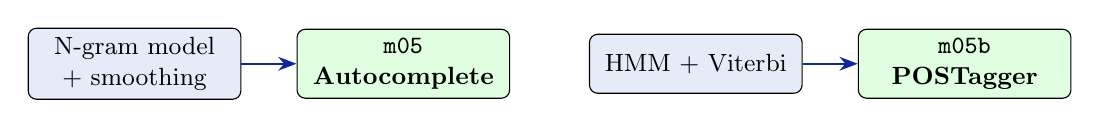
\begin{tikzpicture}[
      mod/.style={draw, fill=cnubluebg, rounded corners=3pt,
                  minimum width=2.7cm, minimum height=0.75cm,
                  font=\small, align=center},
      fin/.style={draw, fill=green!12, rounded corners=3pt,
                  minimum width=2.7cm, minimum height=0.75cm,
                  font=\small\bfseries, align=center},
      arr/.style={-{Stealth}, thick, color=cnublue}
  ]
    \node[mod] (ng)  {N-gram model\\ + smoothing};
    \node[fin, right=0.7cm of ng]  (au) {\texttt{m05}\\ Autocomplete};
    \node[mod, right=1.0cm of au]  (hm) {HMM + Viterbi};
    \node[fin, right=0.7cm of hm]  (po) {\texttt{m05b}\\ POSTagger};
    \draw[arr] (ng)--(au);
    \draw[arr] (hm)--(po);
  \end{tikzpicture}
  \end{center}
  \vspace{5pt}
  \begin{columns}[T]
    \begin{column}{0.50\textwidth}
      \textbf{P5 da qurasiz:}\\[3pt]
      \small
      \begin{itemize}\setlength\itemsep{2pt}
        \item \texttt{m05 Autocomplete}: bigram + add-1, \texttt{perplexity}
        \item \texttt{m05b POSTagger}: HMM + \texttt{viterbi}
        \item Eng ehtimoliy davom va teg ketma-ketligi
      \end{itemize}
    \end{column}
    \begin{column}{0.46\textwidth}
      \textbf{Birinchi assert (bu slayd [I4]):}\\[4pt]
      \small\ttfamily
      assert abs(delta\_VB\_t2\\
      \phantom{assert }- 0.3402) < 1e-4\\[4pt]
      \normalfont\footnotesize\color{halfgray}
      \textit{\# Ma'ruza L5 [I4]-slayd bilan}\\
      \textit{\# solishtiring; yo'l == [NN, VB]}
    \end{column}
  \end{columns}
\end{frame}

% ----------------------------------------------------------------
% [R] ADABIYOTLAR
% ----------------------------------------------------------------
\begin{frame}{Adabiyotlar}
  \begin{enumerate}\small\setlength\itemsep{5pt}
    \item Rabiner, L.R.\ (1989). \textit{A Tutorial on Hidden Markov Models...}
          Proc. IEEE 77(2):257--286.
    \item Jurafsky, D., Martin, J.H.\ (2023). \textit{Speech and Language
          Processing}, 3-nashr. 3-bob: N-gram LM; 8-bob: POS, HMM.
    \item Shannon, C.E.\ (1948). \textit{A Mathematical Theory of Communication.}
          (Til modellashtirish va entropiya ildizi.)
    \item Chen, S., Goodman, J.\ (1999). \textit{An Empirical Study of Smoothing
          Techniques for Language Modeling.} Computer Speech \& Language.
    \item \texttt{nltk.lm} hujjatlari --- N-gram til modellari.
  \end{enumerate}
\end{frame}

% ================================================================
% [S] ILOVALAR (appendix --- slayd soniga kirmaydi)
% ================================================================
\appendix

\begin{frame}{Ilova S1: log fazoda Viterbi (underflow yechimi)}
  \small
  Ko'paytma o'rniga logarifmlar yig'indisi:
  $$ \log \delta_t(j) = \max_i\big[\log\delta_{t-1}(i) + \log A(j\mid i)\big] + \log B(o_t\mid j) $$
  \bunda{$\max$ va $\arg\max$ tartibi log monoton bo'lgani uchun saqlanadi.}
  \vspace{4pt}

  Misol ($t{=}2$, VB): $\log\delta_2(\text{VB}) =
  \max(\log 0.63 + \log 0.6,\; \log 0.03 + \log 0.7) + \log 0.9$.
  Bu $\ln 0.3402 \approx -1.078$ ga teng --- xuddi shu natija, lekin
  underflowsiz.
\end{frame}

\begin{frame}{Ilova S2: perplexity va entropiya bog'liqligi}
  \small
  Perplexity --- model kross-entropiyasining eksponentasi:
  $$ \mathrm{PP}(W) = 2^{H(W)}, \qquad H(W) = -\tfrac{1}{N}\sum_{i} \log_2 P(w_i\mid w_{i-1}) $$
  \bunda{$H(W)$ --- o'rtacha kross-entropiya (bit/token).}
  \vspace{4pt}

  Intuitsiya: agar model har qadamda $k$ ta teng ehtimolli variant orasidan
  ``tanlayotgan'' bo'lsa, $\mathrm{PP}=k$. Shuning uchun perplexity ni
  ``o'rtacha tarmoqlanish koeffitsiyenti'' deb o'qish mumkin.
\end{frame}

\end{document}
